\documentclass{article}
\usepackage{import}
\subimport{../}{preamble}
\begin{document}

%\fullcite{bharadwaj2009}

\section{Plasmons in Tips}
\label{sec:tip_literature}

Significant efforts have been made to advance surface characterisation on the nm-scale by developing new optical tools and integrating optics into existing nanoscale topological measurements. Metallic tips were  investigated due to the widespread use of \glspl{spm}, such as \gls{afm}, and \gls{stm}. The similarity in size between metallic nanostructures and the sub-wavelength size apex of tips initially suggested that visible plasmons would be expected, enabling resonant near-field enhancement. Prior to any spectral characterisation studies to understand the near-field response, tips were applied in combined SPM-optical microscopes to achieve sub-wavelength localisation and enhancement of optical signals. As the next logical step from \gls{sers} and \gls{snom}, the sharp apex of tips were exploited to develop the spin-off techniques of \gls{ters} \cite{stockle2000, anderson2000, hayazawa2000, pettinger2000} and \gls{asnom}%
\footnote{Also known as \gls{ssnom}.}
\cite{zenhausern1994, zenhausern1995, bachelot1995, knoll1997, knoll1998, keilmann1999}.
These are also known collectively as \gls{tenom}.%
\footnote{These are also sometimes known as field-enhancing near-field optical microscopy (FENOM) since apertured techniques do not necessarily exploit plasmonic enhancement as much.}

% TERS
The concept for \gls{tenom} was first proposed in 1985 \cite{wessel1985} but it was not until 2000 that the first reported uses of tips for enhancing Raman spectroscopy emerged \cite{stockle2000, anderson2000, hayazawa2000, pettinger2000}. All measurements were carried out in inverted microscopes with either an \gls{afm} \cite{stockle2000, anderson2000, hayazawa2000} or \gls{stm} \cite{pettinger2000} mounted on top. Two of the initial measurements suggest the overall Raman enhancement has a lower limit of $\sim$\num{e4} \cite{stockle2000, anderson2000}, hence a field enhancement \orderof{10}. A third independent measurement utilising evanescent wave excitation obtained an enhancement factor of 80 from a single tip apex, equivalent to the summed enhancement of many SERS hotspots on a Ag island film \cite{hayazawa2000}. Since then Raman enhancements in the region of \num{e7}--\num{e9} have been measured \cite{pettinger2012}.%
\footnote{A clear distinction is made between the field enhancement, $|E/E_0|$, and the Raman enhancement, $|E/E_0|^4$, when stating enhancement factors. In the literature the terms ``field enhancement" or ``enhancement factor" are generally used interchangeably between the magnitude of the near-field and the improvement in the Raman signal.}
Whilst SERS enhancement factors have also increased significantly in recent years, the \gls{tenom} approach to spectroscopy remains popular since the tip can be scanned across a sample. For this reason, techniques such as TERS are widely considered to become the successors of SERS. However, for this to be the case, nanotips require the capability to controllably and reproducibly enhance the near-field. Understanding the electromagnetic response of metallised tips has therefore become of significant importance in recent years.
Since the use of tips for observing fundamental plasmonics is also a central part of this project it becomes important to understand the underlying concepts and mechanisms of \gls{tenom} as these inevitably influence any observed plasmonic behaviour.

\begin{figure}[bt]
%\centering
\flushleft
\begin{subfigure}[t]{0.47\textwidth}
	\subimport{./figures/}{tenom_basic}
\end{subfigure}
~
\begin{subfigure}[t]{0.49\textwidth}
	\subimport{./figures/}{tenom_surface}
\end{subfigure}
\caption[Concepts of TENOM]{\textbf{Concepts of TENOM.} Basic TENOM systems constitute a tip and a sample (left). Tips can perturb evanescent surface waves, generated by high-\NA\ TIR, and scatter them into the far-field ($1\rightarrow3$) \cite{neacsu2005, mehtani2006}. Photons illuminating the tip can induce a weak dipole localised to the tip apex, which can scatter the near-field ($2\rightarrow3$). More recent TENOM arrangements employ a metallic substrate to couple with the tip and further localise the field into a ``hot spot" (right). Coupling of plasmons between the tip and the substrate can be achieved by exciting SPPs on the substrate using evanescent waves (1) or by focusing light on the MIM gap such that the tip dipole induces an image dipole in the substrate (2). Both mechanisms lead to scattering of light from the gap into the far-field (3). SPPs generated onto the planar surface (either via the tip or evanescent waves) can radiatively decay into $\mathit{NA}>1$ ($1,2\rightarrow4$) \cite{wang2011}.}
\label{fig:tenom_concept}
\end{figure}

\Gls{tenom} is ideally classified as a local excitation approach as opposed to a local scattering approach \cite{novotny2006}, though the two are not independent. \figurename~\ref{fig:tenom_concept} shows the general approaches to \gls{tenom}. In the tip scattering approach the non-radiative near-field, comprising evanescent waves, is perturbed by the presence of the tip, leading to scattering into the far-field {\color{red}(same frequency as illumination but lower \wvm)}. In the tip excitation approach the tip is resonantly excited to induce a large, local, near-field enhancement and used as a sub-diffraction-limited light source, from which  localised scattering can be measured. This process can be much more efficient than the pure scattering approach but depends on the optical antennae properties of the tip. In both cases the resolution of scattering images is sub-diffraction limited and set by the size of the tip radius ($\sim$\SI{50}{nm}).

\subsection{The Electromagnetic Response of Tips}

\begin{wrapfigure}{O}{0.45\textwidth}
\centering
\vspace{-15pt}
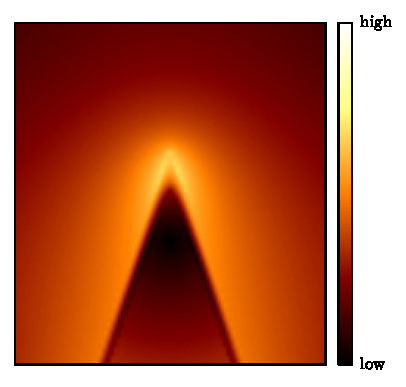
\includegraphics[width=\textwidth]{figures/lightning_rod_effect}
\vspace{-25pt}
\caption[Calculated magnitude of the electric field around a tip showing the lightning rod effect]{\textbf{Calculated magnitude of the electric field around a tip showing the lightning rod effect.} Compression of the field lines around the sharp corner of an equipotential surface leads to a localised, non-resonant field enhancement.%
\footnote{Poisson's/Laplace's equation is solved for a tip structured electrode with a surface charge distribution separated by some distance from a planar metal counter electrode of the opposite surface charge.}}
\label{fig:lightning_rod_effect}
\end{wrapfigure}

The electromagnetic response of tips can be broken down into individual components that constitute the enhancement mechanism. The two main optical components are the lightning rod effect and a resonant plasmon contribution for metallic tips \cite{esteban2006, zhang2009, schmid2013}. Each component is maximised when the incident field is along the tip axis \cite{zhang2014}. The main focus of recent tip work has been to study the plasmonic component, however progress in sharpening tips has led to increases in the lightning rod component. Both components are important to consider when attempting to understand optical measurements involving tips.

% The lightning rod effect in tips
Regardless of plasmonic behaviour, metallic tips intrinsically exhibit a lightning rod effect under the application of an applied field, instilling a non-resonant component of near-field enhancement. From the definition of the electric field $\vec{E}(\vec{r}) = -\nabla\pot(\vec{r})$ it is clear that the electric field strongly depends on geometry, with field lines perpendicular to the equipotential conductor surface. The more curved a surface, the more compressed the field lines become around its surface due to accumulation of surface charge. This can be described by $E = \sigma/\epsfs$ where $\sigma = q/4\pi r^2$ is the surface charge density and $r$ is the radius of curvature. Since $E \propto 1/r^2$ the electric field is larger in regions of smaller curvature, as shown by the simple model in \figurename~\ref{fig:lightning_rod_effect}. Consequently, even without a plasmonic component, sharp tips provide a promising platform for localised near-field enhancement.

% The plasmonic component
The expected plasmonic component also arises from the curvature of the metal-dielectric interface at the tip apex. Curvature allows for both \gls{spp} excitation and \gls{spp} localisation at the apex due to adiabatic nanofocussing \cite{stockman2004, pile2006, berweger2010, lee2011, berweger2012, lindquist2013}. As highlighted when discussing ellipsoidal \glspl{mnp}, strong, antenna-like \glspl{lsp} are unlikely to be excited at the apex of a sharp tip since lack of a second metal-dielectric interface prevents accumulation of the opposite surface charge to the apex. The tip can almost be described as a MI geometry as opposed to the \gls{imi} geometry that results in antenna-like \glspl{lsp}. Thus there can be no strong restoring forces or \glspl{spr}. The extended size of the typical tip structure ($\sim$\SI{20}{\micro\metre}) also means that any potential low-order antenna modes would exist in the IR. Calculations for shorter tip geometries (nanocones or nanoellipsoids) show visible-NIR \glspl{lsp} \cite{roth2006, goncharenko2006}, however these redshift and diminish with increasing tip length \cite{zhang2009, huber2014}. The standard, sharp metallic tip geometry therefore makes for a poor \textit{plasmonic} optical antenna unless \glspl{spp} can be excited.

Despite this claim, a large number of publications give convincing evidence for the presence of localised apex plasmons, such as TERS background resonances \cite{pettinger2007, pettinger2009} and depolarised scattering images \cite{mino2014}, however the tips used typically have a degree of nanostructuring allowing more localised modes \cite{hayazawa2001, bailo2008, hayazawa2012, mino2014}. These localised components of the plasmonic tip contribution are generally reported to originate from surface roughness imparted by the coating procedure, mimicking small 10--\SI{50}{nm} \glspl{mnp} \cite{mino2014}. Similar behaviour has been used to explain the origin of \gls{sers} in rough metal films. Each grain of the coating acts as a point at which photons couple and plasmons radiate, hence a grain located at the apex can plasmonically enhance and scatter the near-field. For this reason sharp tips are generally all solid etched metal or metallised dielectric tips, coated using evaporation (with similar conditions to metal island deposition) \cite{hayazawa2001, hayazawa2012, mino2014} or chemical reactions \cite{bailo2008}.

In general there is the consensus that tips, in some way, support both \glspl{spp} and \glspl{lsp}, which, under different conditions, contribute to the overall near-field enhancement with differing degrees of magnitude. More work is needed to fully understand and optimise the tip geometry to gain the most from enhancement. 
% Maybe work on that last paragraph
Alternatively the tip is coupled with a planar metallic substrate to effectively form a plasmonic \gls{mim} cavity, enabling localised gap modes \cite{ren2004, neacsu2006, hayazawa2007, yano2007, pettinger2009, uetsuki2012, lindquist2013}. In this instance, a weakly-excited dipole in the tip can induce an image dipole in the metallic surface to form a strongly-confined coupled gap mode. Coupling can be achieved by either exciting the tip dipole or by using \gls{spp} excitation on the underlying metallic substrate \cite{hayazawa2007}. Unlike the coupling between \gls{mnp} plasmons, theory suggests that the coupling between a Au tip and a Au surface only minimally shifts the gap resonance \cite{downes2006}.

% Theory work
%\cite{Demming2005, Rogov2013, behr2008}
Complete theoretical understanding of these effects is challenging due to difficulty in modelling tips. Their sub-wavelength apices and large (\SI{20}{\micro\metre}) overall conical or pyramidal structure lead to complications when simulating their response, and approaches attempting to circumvent these limitations often cause physical inaccuracies in the result.
%Potential inaccuracies include unphysical modes caused by interference of reflected \glspl{spp} around the tip surface and charge accummulation on non-physical interfaces.
Incredibly simplistic models, such as modelling only the tip apex, usually as a spherical or ellipsoidal \gls{mnp}, fail to take into account the actual tip geometry, resulting in the existence of unphysical \gls{mnp}-like modes at the tip apex. Similar multipolar modes are exhibited by tip models with finite lengths less than \SI{1}{\micro\metre} \cite{roth2006, goncharenko2006}, behaving more like nanopyramids \cite{schafer2013, cherukulappurath2013}. Realistic excitation of geometrical (spherical) \gls{lsp} resonances at the apex, similar to those in \glspl{mnp}, have weak dipole moments as a result of the singular metal-dielectric interface and are therefore far less radiative than \glspl{mnp} \cite{downes2006}. {\color{red}The lack of radiative lower order multipolar resonances greatly diminishes the radiative cross section \cite{renger2004}.} Recent models accounting for the actual tip length show the disappearance of such modes into a smooth continuum as the tip is continually lengthened \cite{zhang2009}.

Zhang \emph{et al.} \cite{zhang2009} suggest that between lengths of \SI{200}{nm} and infinity a tip transitions between supporting low order \glspl{lsp}, then higher order \glspl{lsp}, followed by only weak \glspl{spp}. \Glspl{lsp} are supported only when the entire tip structure is smaller in size than the focus, allowing light to drive in-phase collective oscillations of the conduction electrons. As the tip becomes larger, phase retardation occurs and higher order \gls{lsp} modes dominate. Once the tip becomes larger than the focus, the case for almost all \gls{spm}-based tips, collective oscillations are no longer possible, leaving only weak \glspl{lsp} concentrated at the apex surface and \glspl{spp}. \Glspl{spp} form a periodic response in the field enhancement before disappearing due to increased losses with increasing tip length. The field enhancement then rises smoothly and non-resonantly towards the IR as only a lightning rod contribution remains and the relative apex sharpness compared to the illumination field increases with wavelength. Interestingly, Zhang \emph{et al.} further show that a sharp tip with a \SI{10}{nm} radius cannot compete with the enhancements brought on by collective \gls{lsp} excitation in a broader radius structure. % check this

%Calculations of a Au tip approaching a Au surface, considering only the apex region (adaptive meshing), in the quasi-static approximation \cite{behr2008}. By considering only the quasistatic regime the Laplace equation can be analytically solved, simplifying the computation time and giving greater insight into the physical quantities and how they behave. However, this approach assumes a plasmon exists at the apex with no method of optical excitation other than evanescent wave coupling.

%{\color{red}Despite using an apex-localised, quasi-static model to analytically predict the spectral response of tips and tip-sample interactions, a visible frequency plasmon resonance ($\sim\SI{550}{nm}$) is calculated for a hyperbolic tip, one which is independent of cone angle, which only affects the field enhancement, but sensitive to tip radius (redshifts with decreasing radius) and gap coupling with a planar surface \cite{behr2008}. As with any quasi-static model phase retardation is neglected meaning it is not possible to predict multipolar resonances. While this model shows agreement with FTDT calculations \cite{} and early experimental measurements \cite{neacsu2005} the specific conditions required to excite the LSP are not discussed.

Even with the frequent recent use of \gls{tenom} there has been few reports experimentally measuring the optical response of tips or characterising their spectra prior to use, for example, in \gls{ters}. The first direct observation of tip plasmons was in 2005. Scattering of evanescent waves at the surface of a prism by a metallic tip was used to measure the near-field response in Au and W tips \cite{neacsu2005}. The 600--\SI{800}{nm} spectral resonance present in Au, but not W, was attributed to excitation of \glspl{spp} at the tip apex. Two separable $s$ and $p$-polarised modes were extracted from the plasmonic Au spectra showing the expected anisotropy along each of the tip axes.
% \cite{Neacsu2006} also shows spectrum and image coupling
Further measurements of evanescent field scattering by metallic tips have shown similar results \cite{mehtani2006, barrios2009}. Shifts of $\sim$75--\SI{100}{nm} have been observed between Ag and Au tips with a Si\subs3N\subs4 underlying tip material redshifting resonances by $\sim$\SI{30}{nm} compared with solid metallic tips. This dependence on tip structure has been highlighted numerous times due to the two dominant tip geometries of sharply etched metal tips and metallised (metal-coated) non-metallic tips.

\subsection{Challenges associated with Tip-based Near-Field Microscopy}

\begin{figure}[bt]
\centering
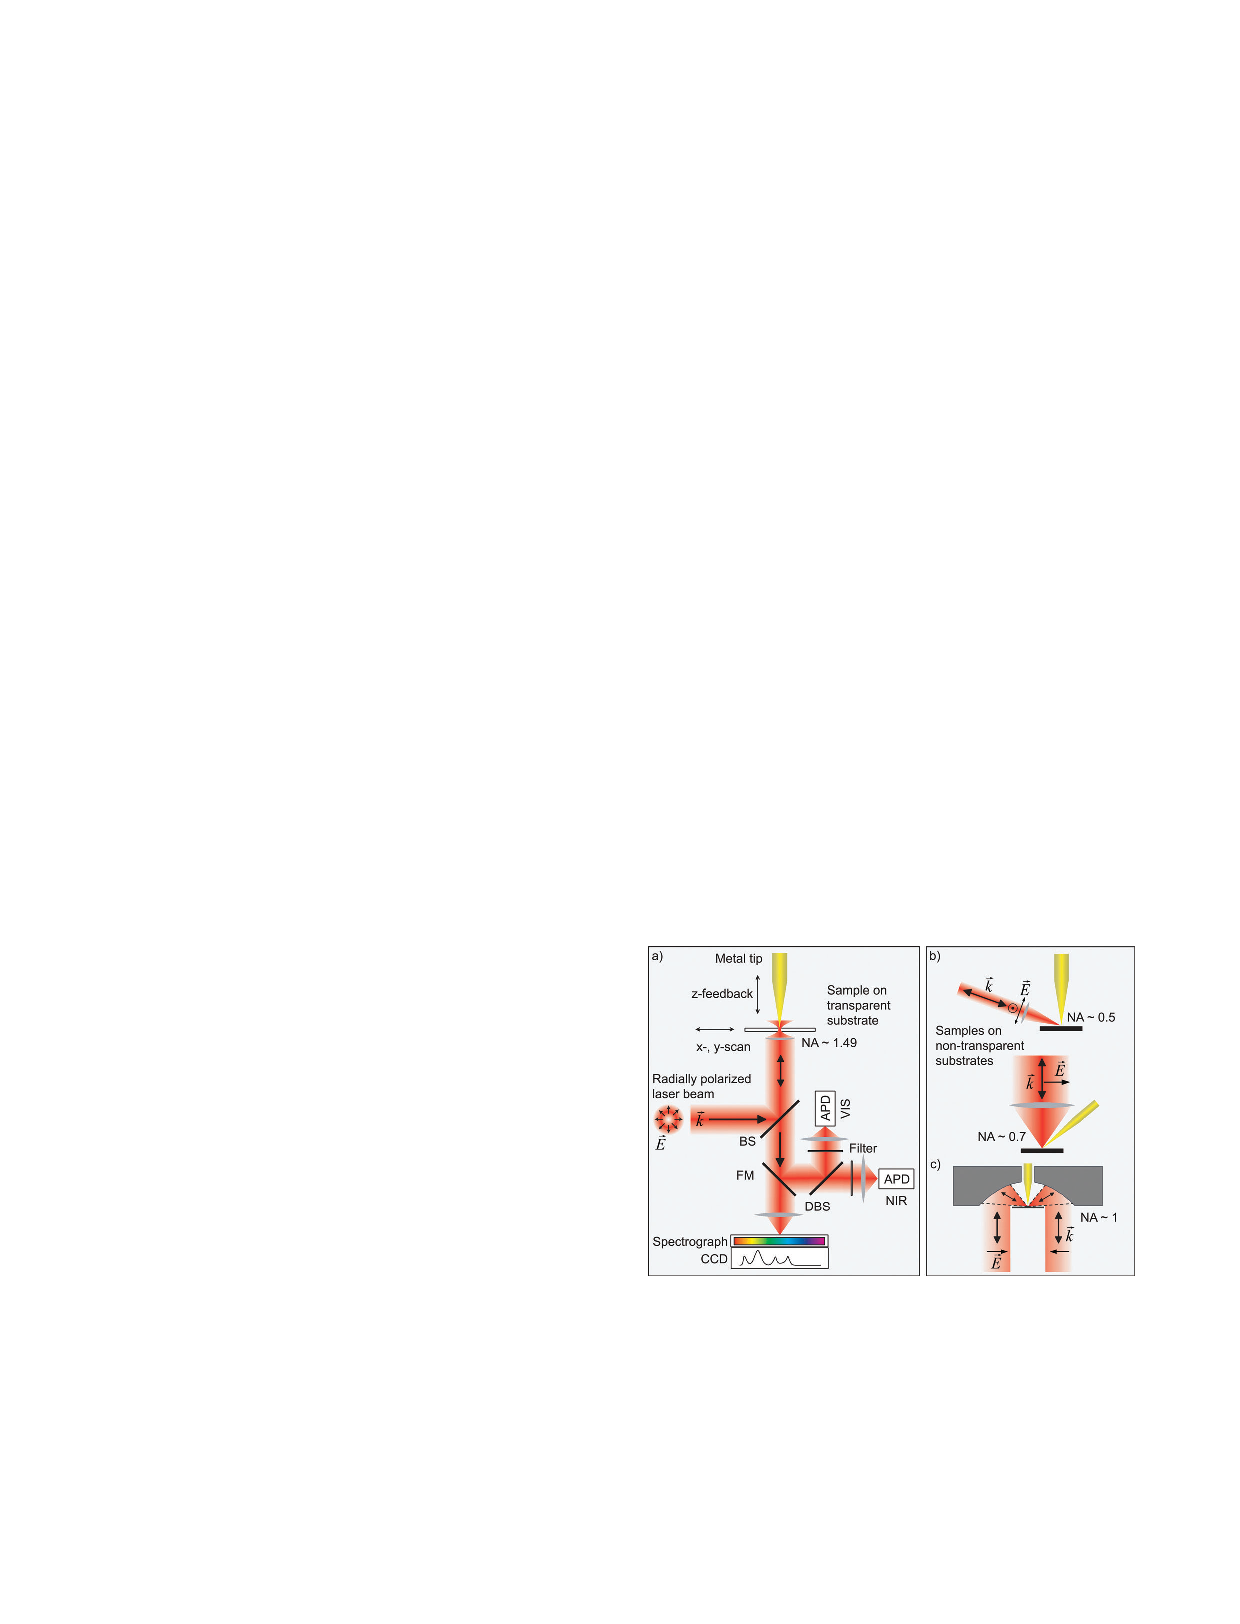
\includegraphics[width=0.6\textwidth]{figures/literature/mauser2014a}
\caption[Typical optical geometries found in TENOM experiments \cite{mauser2014}]{\textbf{Typical optical geometries found in TENOM experiments \cite{mauser2014}.} The most prominent system is the bottom-illumination/back-illumination configuration utilising high-NA objectives. The other main geometry is the side-illumination configuration.}
\label{fig:ters_geometries}
\end{figure}

Since initial investigations, tip-based systems have been designed in two configurations: the side-illumination and bottom-illumination configurations. Both are shown in \figurename~\ref{fig:ters_geometries}. The specific design of a \gls{tenom} microscope is important as it defines the collection and, more importantly, excitation geometries for the tip. Continuous wave illumination is generally used though ultrafast systems have been exployed to extract temporal information from measurements \cite{klingsporn2013}.

Side-illumination has been used successfully in a number of cases \cite{mehtani2006, zhang2013, wickramasinghe2014} but suffers generally from far-field scattering overshadowing the near-field scatter. This requires more complex optical geometries to overcome, such as using polarisation-resolved or interferometric approaches. More recent designs have opted for a side-illumination geometry, in which high NA is achievable by using parabolic reflectors instead of an objective lens \cite{steidtner2007}. In each case, side-illumination can be classified as a far-field excitation technique.

The dominant microscope design is the bottom-illumination configuration, using $\NA>1$ illumination and \gls{tir} to excite the tip evanescently. \Gls{tir} results in minimal background scatter with only the near-field scattered into a collection aperture. Collection from this geometry can be achieved using either the $\NA<1$ aperture of the high \NA\ illumination objective \cite{hayazawa2001, yeo2006, yeo2007, zhang2013experimental, mino2014, kumar2014} or a secondary low NA objective \cite{hayazawa2007, taguchi2009, uetsuki2012}. More importantly, evanescent waves generated by bottom-illumination can couple to \glspl{spp} in both a metallic substrate and the tip once it is within the near-field. This does, however, require that samples are optically transmissive, which is not always possible. For these reasons it is important to consider the optical geometry when understanding the results presented from a study.

\begin{figure}
\centering
\fcapside[\FBwidth]
{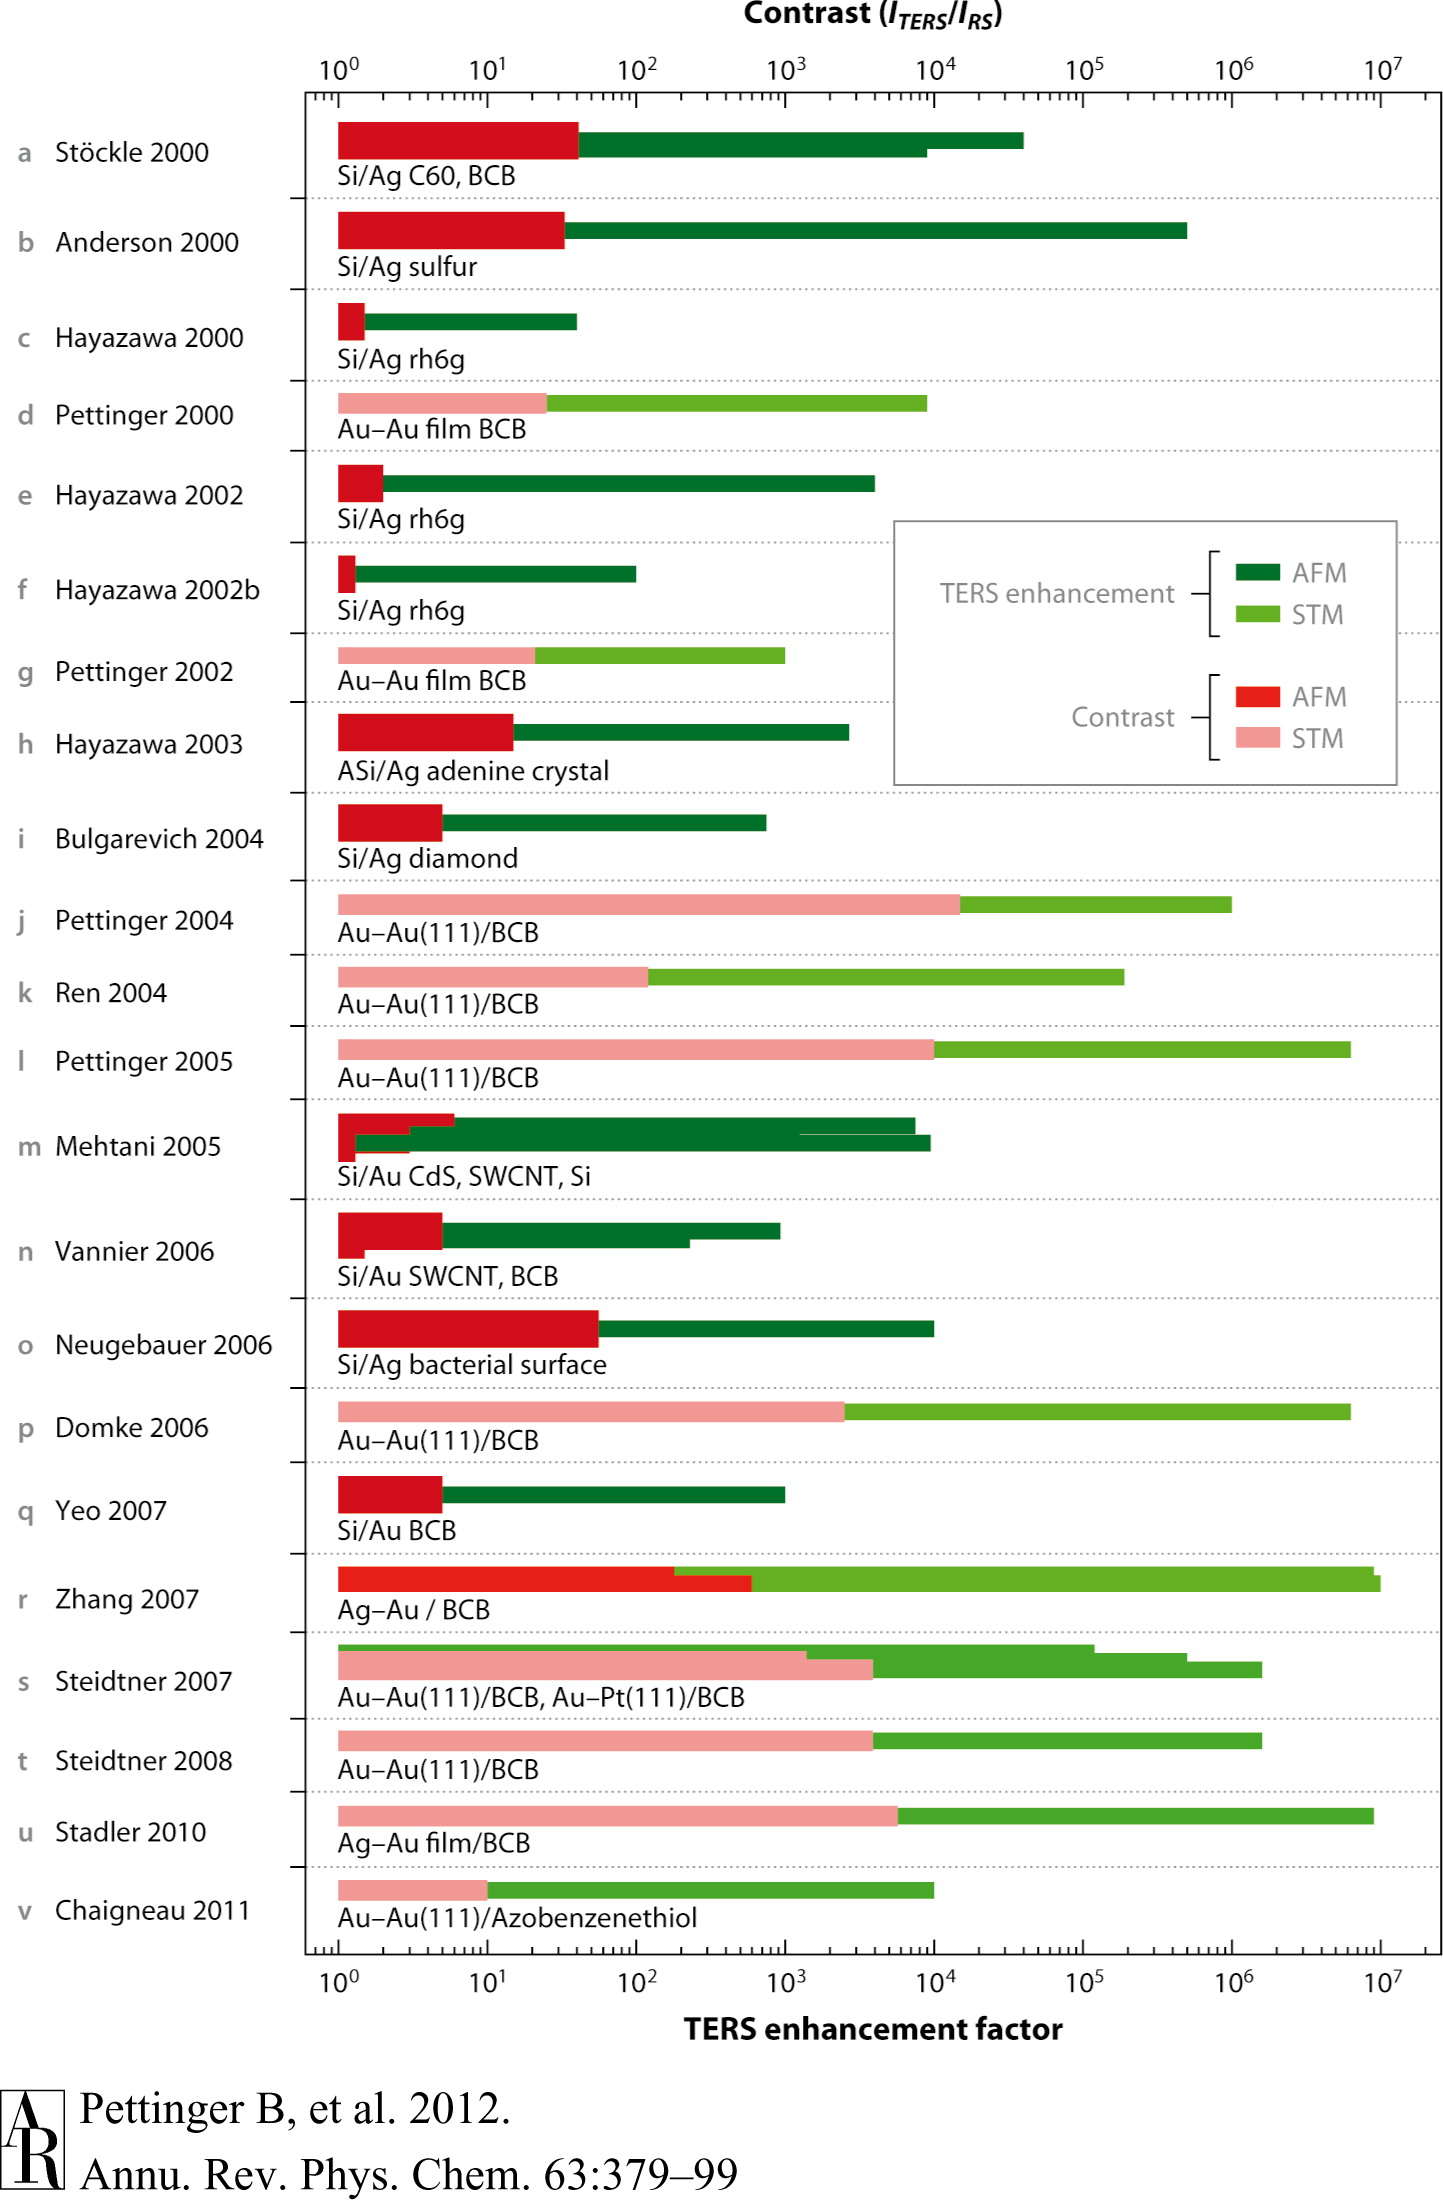
\includegraphics[width=0.7\textwidth, clip=true, trim=0 35 0 0]{figures/literature/pc630379_f8}}
{\caption[Comparison of TERS field enhancements and contrasts reported between 2000 and 2011 \cite{pettinger2012}]{\textbf{Comparison of TERS field enhancements and contrasts reported between 2000 and 2011 \cite{pettinger2012}.} STM tips, likely due to their increased sharpness, outperform AFM tips. Ag tips outperform Au tips. Larger enhancements are observed in systems where there is an underlying thin, noble metallic film. Statistical correlations still remain somewhat weak, showing the current variability in TERS experiments, attributed to irreproducibility of enhancing tips.}
\label{fig:pettinger2012}}
\end{figure}

% Challenges for TERS and comparison between measurements
Since the initial measurements of tip enhancements and plasmons, techniques such as \gls{ters} and \gls{asnom} have become widespread. However, they are currently not reliable enough to be considered as a standard technique. Difficulty controlling the tip near-field is both a result of the irreproducibility of the tip geometry and a lack of understanding of the optical processes governing the enhancement, leading to large variations between reported field enhancements and \gls{ters} contrasts. A selection of these, reported between 2000 and 2011, are shown in \figurename~\ref{fig:pettinger2012}, showing the variability of \gls{ters}. The current challenges with \gls{tenom} are therefore improving the reproducibility of the near-field enhancement between tips \cite{blum2014, kumar2014, mino2014} and successful electromagnetic modelling and understanding of the tips themselves \cite{zhang2009}. % check this reference

% Sharpness and lightning rod effects
Factors determining the efficiency of \gls{tenom} include experimental excitation/collection geometry, tip sharpness, surface metal morphology, material influences and tip/apex orientation. From \figurename~\ref{fig:pettinger2012} it is clear that sharper \gls{stm} tips result in larger field enhancements than metallised \gls{afm} tips and comparative studies have shown similar trends \cite{raschke2003, yeo2006, picardi2007}. This intuitively suggests that the lightning rod effect plays a significant role in the near-field enhancement process. However, sharpness-induced enhancements can only be improved to a point as recent theory indicates there is a quantum limit set by nonlocal effects, at which point the enhancement saturates as the field becomes smoothed around any finer structural imperfections \cite{wiener2012}. Understanding how to optimise the plasmonic component in tips is therefore a priority.
%Studies have also shown that some large observed enhancement factors can be caused by non-plasmonic artefacts from the tip shaft \cite{ramos2012}. Removal of these artefacts is necessary to recover the actual near-field enhancement \cite{kumar2014}.

% Material dependence
Materials choice, as with much of plasmonics, heavily influences any plasmonic behaviour. As with many other plasmonic structures, Ag tips generally outperform Au tips under visible light, although these claims are highly dependent on the underlying tip material and metal morphology. Only the metal morphology is important in solid \gls{stm} tips and thickly metallised \gls{afm} tips, where plasmon energies are unchanged regardless of any potential underlying materials. On thinly coated ($<\SI{40}{nm}$) \gls{afm} tips, plasmon are tuned by the metal film thickness \cite{huber2014} and the refractive index of the underlying tip material, which can vary drastically between materials such as Si, SiO\subs2, and Si\subs3N\subs4 \cite{picardi2007, taguchi2009}. These high index materials can shift any \glspl{spr} into the infrared. Careful consideration must therefore be given when pairing a tip with a laser in order to match the excitation wavelength with the \gls{spr} \cite{yeo2006, yeo2007, cui2007, hayazawa2012}.

% Plasmonic component
\begin{figure}[bt]
\centering
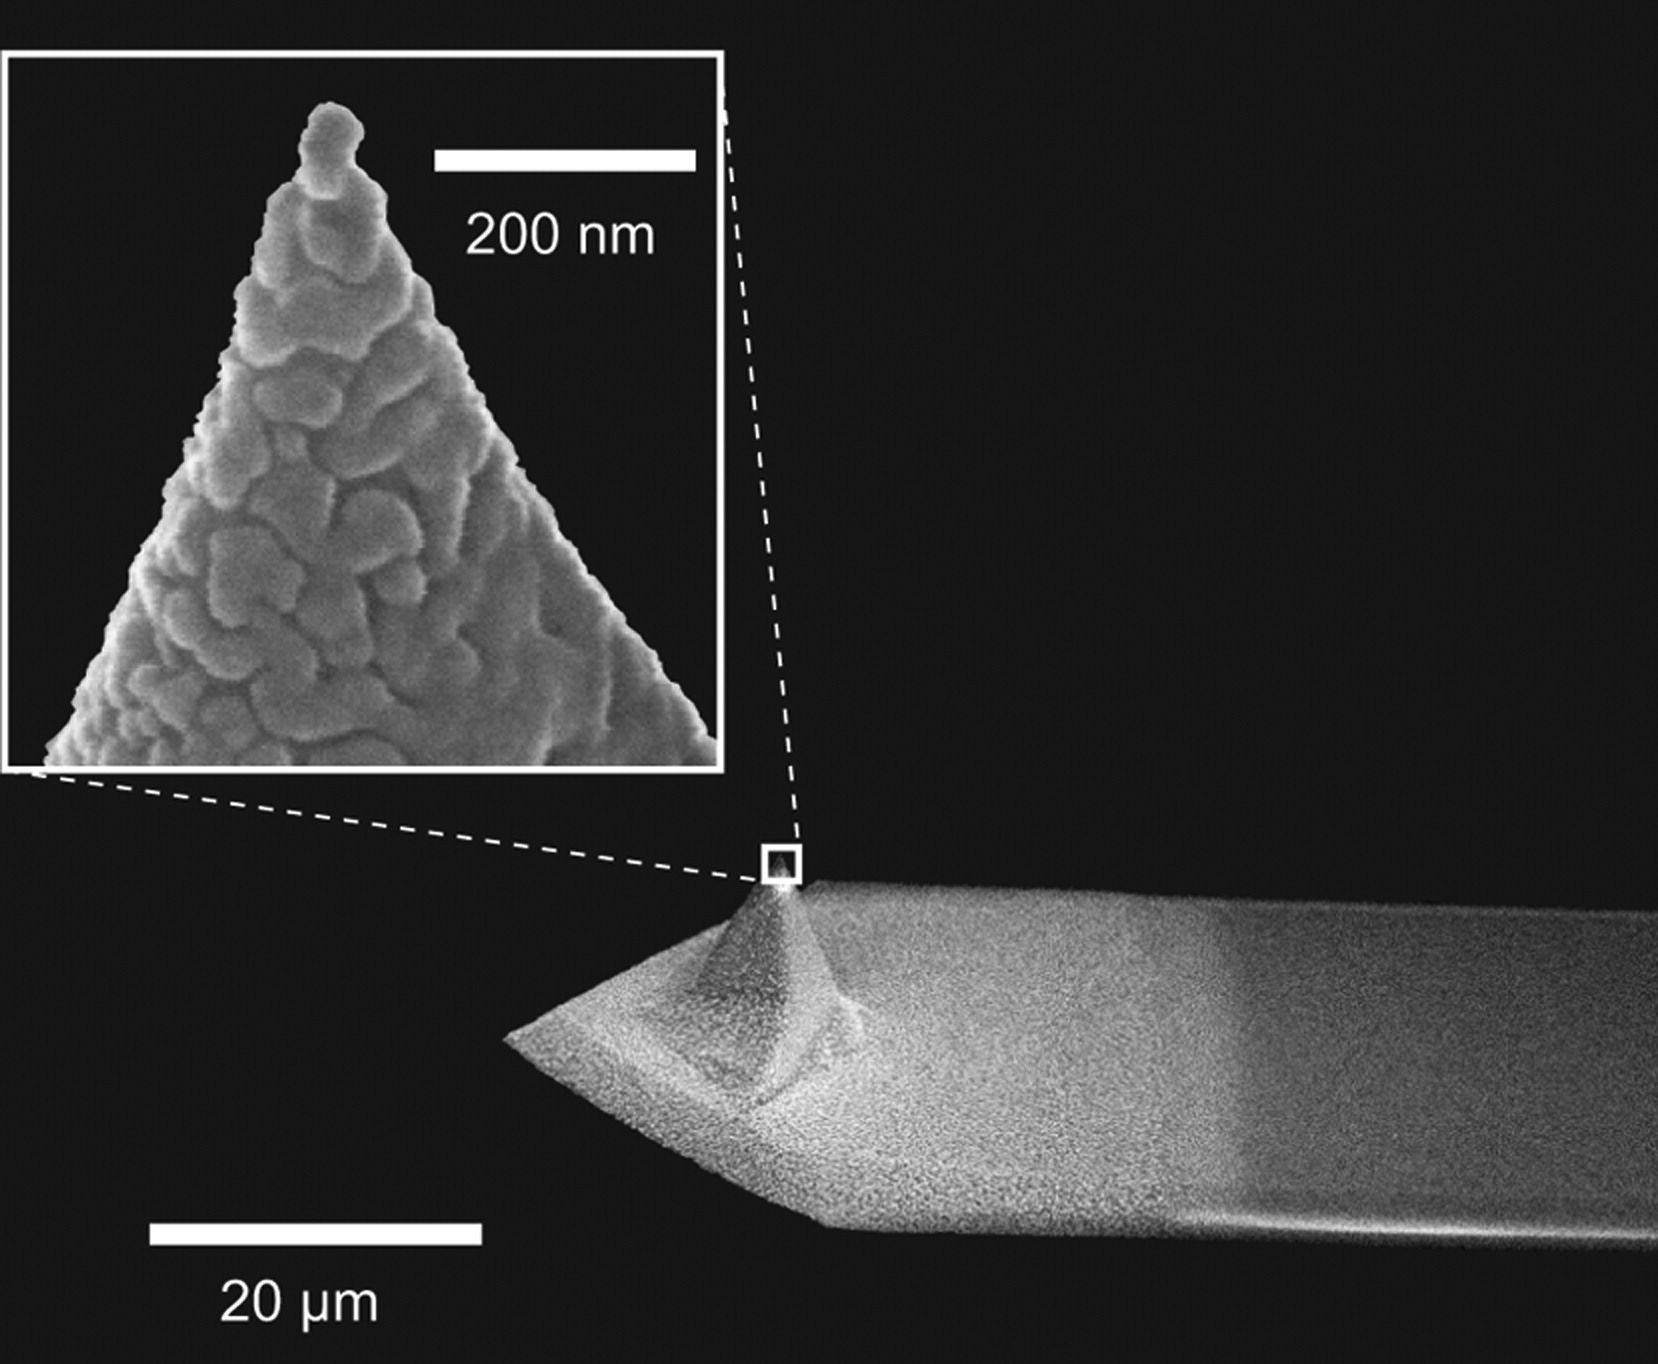
\includegraphics[height=5cm, clip=true, trim=5 75 113 10]{figures/literature/nn-2014-031803_0002}
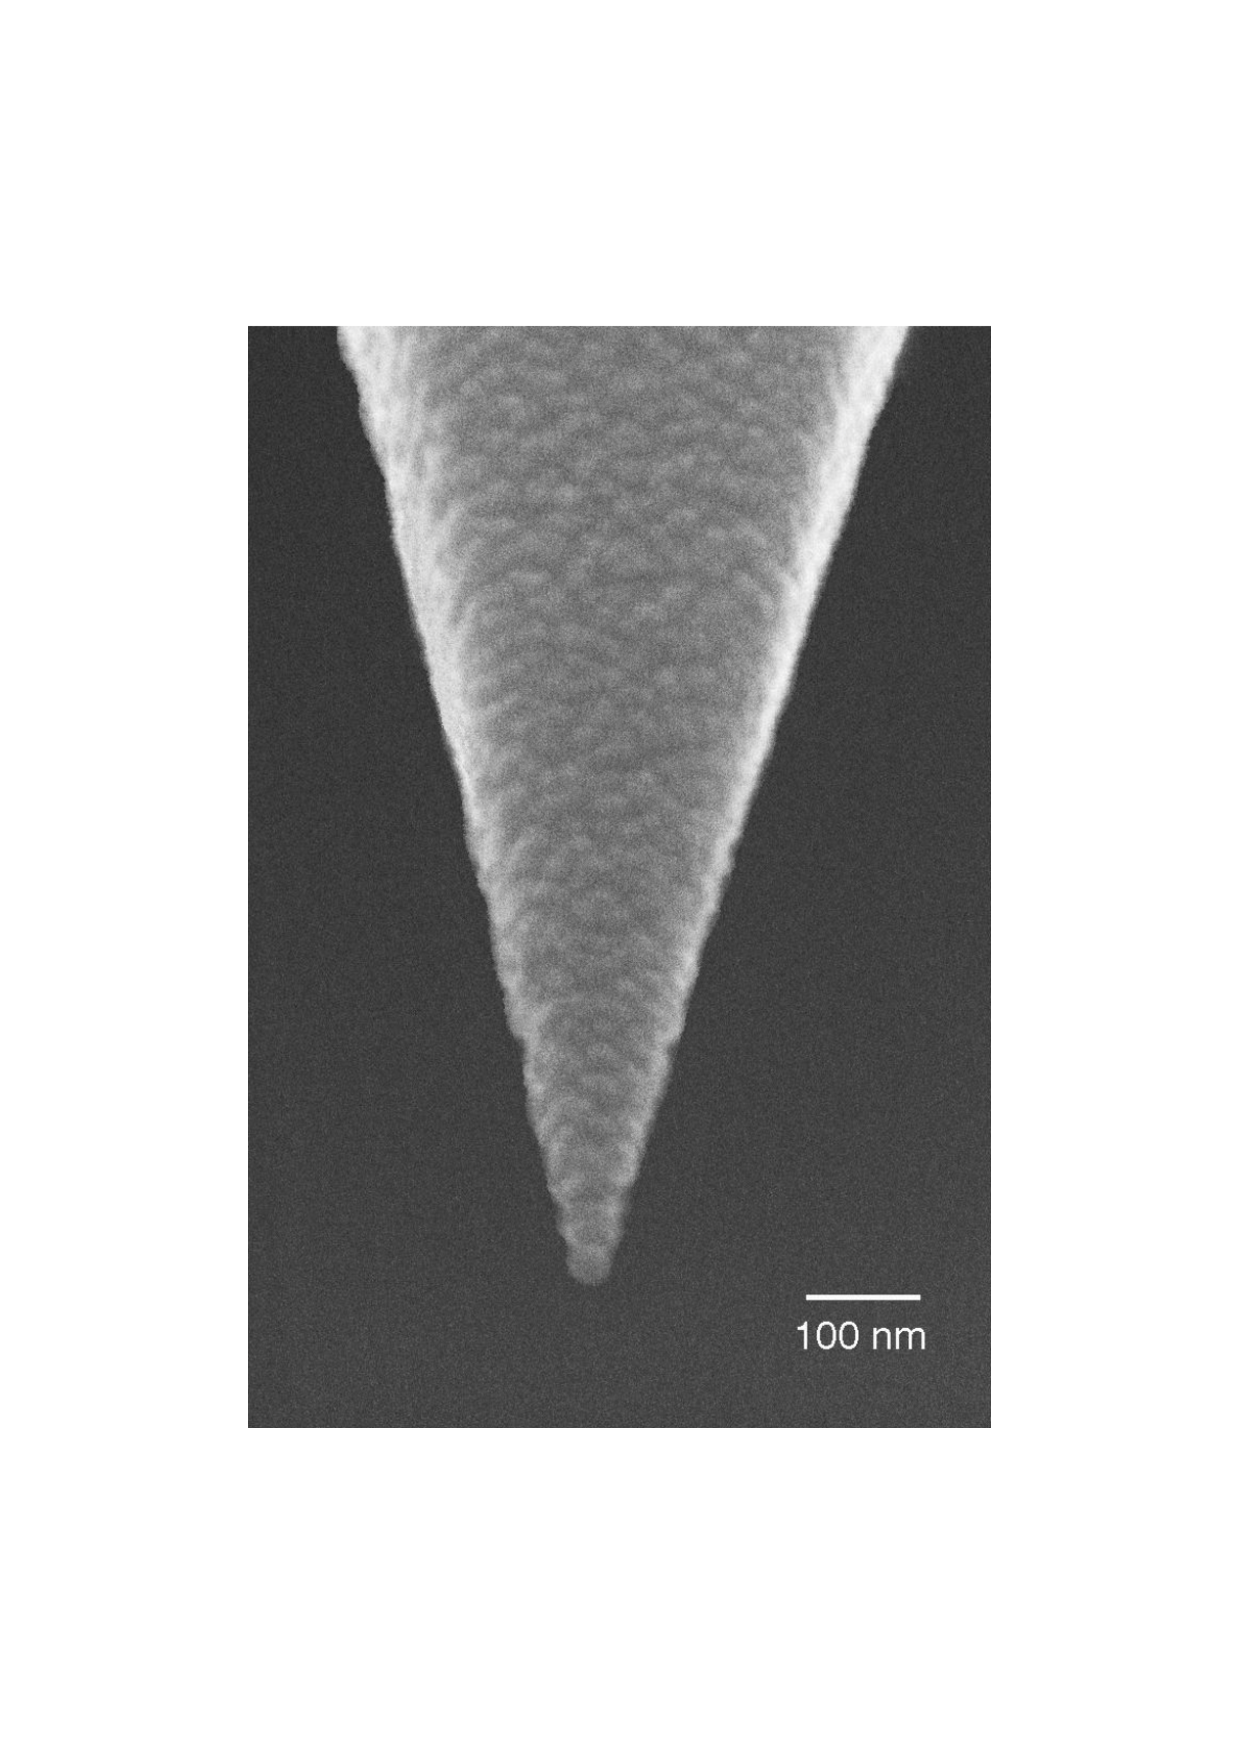
\includegraphics[height=5cm, clip=true, trim=170 180 140 280]{figures/literature/uetsuki2012supp}
%\includegraphics[width=0.3\textwidth, clip=true]{figures/literature/1-s2-0-S0009261401000653-gr1}
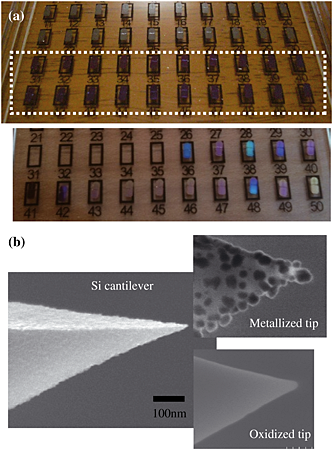
\includegraphics[height=5cm, clip=true, trim=20 5 0 165]{figures/literature/jrs4032-fig-0001}
\caption[]{\textbf{SEM images of metallised tips exhibiting random nanostructures.} Images are taken from \cite{mino2014} (left), \cite{uetsuki2012} (middle) and \cite{hayazawa2012} (right). Each SEM shows randomised grains deposited using evaporation. These are thought to enable LSP excitation if located at the apex.}
\label{fig:metallised_tips}
\end{figure}

% Morphology dependence
A large amount of variability stems from surface metal morphology. Reliance on randomised apex geometries, as shown in \figurename~\ref{fig:metallised_tips}, for \gls{lsp} excitation greatly limits reproducibility. Furthermore, this granularity is rarely taken into theoretical account when attempting to explain the mechanisms of \gls{tenom}. The orientation of the tip, along with the roughened apex, with respect to the sample and the incident excitation field also influences near-field enhancement \cite{yeo2006, mino2014}.

Larger enhancements have resulted from coupling with thin metallic substrate films, suggesting the formation of gap plasmons \cite{ren2004, hayazawa2007, yano2007, pettinger2009, uetsuki2012}. Specifically, when a Au tip is paired with a Au substrate the field enhancement is significantly increased, moreso than when paired with a Pt surface \cite{ren2004} or a non-metallic surface \cite{downes2006}. This is attributed to better optical polarisability of the Au substrate. In these cases the Raman enhancement has been shown to rise to $\sim$\num{e7}--\num{e9} \cite{uetsuki2012}. % maybe comment more on the mechanism for this excitation as side illumination alone may not be enough i.e. excitation geometry more important than collection. also removed the phrase 'when illuminated on resonance with the gap mode'.

Finally, variability between similar measurements can stem simply from differences in tip placement, optical setup and the specific illumination/collection geometry or optics used. As tips are rarely characterised there is little traceability between measurements from which to systematically determine the relevant causes for difference. It is highly likely, however, that geometrical limitations are the current dominating limitation restricting the progress of \gls{tenom}, leading to research into new tip geometries with better optimised, well-known optical responses.

% Electrical excitation
One final tip-based plasmon excitation mechanism of interest that has been discussed in recent years is electrical excitation. Similar to the use of \gls{eels} in electron microscopy, tunnelling electrons can be used to excite plasmons in an \gls{stm} geometry. Since tips are typically illuminated with a single wavelength of light it becomes difficult to discern plasmonic features hidden in the collected light. Electrical excitation circumvents this limitation as electrons need only to have sufficient energy $eV$ that a portion transferred to the conduction electrons is enough to excite \glspl{sp} with frequencies $h\nu \leq eV$. Electrical excitation also functions to both remove background light contributions to spectra by removing the illumination source.

Using tunnelling current excitation, light has been observed from both the tip-air-metal substrate gap \cite{pettinger2007, pettinger2009} and the interface between the metal substrate and its underlying dielectric \cite{wang2011}. Broad resonances, which redshift with decreasing tip-sample separation, are found superimposed onto \gls{ters} spectra when operating in the \gls{stm} configuration \cite{pettinger2007, pettinger2009}. These suggest the formation of a \gls{mim} gap mode. Light detected from metal-glass interfaces is leakage radiation from \glspl{spp} on the metal-air interface. Since light cannot leak from \glspl{spp} at the metal-air interface the detected light must be scattering from gap plasmons between the tip apex and the surface {\color{red}and outcoupling at the curved surface}. It is thought that 95\% of the emission is due to \gls{spp} excitation rather than \gls{lsp} excitation \cite{wang2011}.
% this causes problems with the idea of antenna modes.

\subsection{Tip Modification, Nanostructuring and Optical Antenna Tips}

% Transitioning the discussion from sharp to nanostructured tips
The mode mismatch caused by the size difference between diffraction-limited light and the nm-scale results in a 3--4 order of magnitude coupling efficiency loss \cite{berweger2010}. As described previously, a \gls{sp} acts as an optical antenna. A good optical antenna has the ability to effectively modify the density of electromagnetic states such that the far-field radiation impedance is efficiently matched with the impedance of a near-field evanescent mode and vice versa \cite{novotny2006, novotny2011}. The antenna opens up scattering pathways between near-field emitters and the far-field by connecting wave states (\wvm-vectors) via new intermediate states (the plasmon). As stated previously, sharp metallic tips, in their standard form, are not particularly good optical antennae. To improve their coupling efficiency, standard sharp tips have been modified or nanostructured to introduce such intermediary plasmon states \cite{mauser2014}. Whilst this is usually achieved by roughening the metal surface, more reliable and reproducible methods have been developed in recent years to controllably nanostructure the tip and engineer the optical response.

% Grating tips as nanoscale light sources
By patterning a grating onto the side of a conical metallic tip, its apex can be transformed into a nanoscale light source, in which \glspl{spp} excited on the grating propagate to the apex and re-radiate into the near-field \cite{neacsu2010}. Far-field illumination remains spatially separated from the apex, suppressing far-field background scatter, allowing only near-field scattering from the apex to be measured. The conditions for adiabatic nanofocussing mean that only a single \gls{spp} mode localises at the apex and radiates. Background-free \gls{ters} signals using the resulting \SI{10}{nm} light source at $\lambda=\SI{800}{nm}$ have been detected to demonstrate the benefits of using \glspl{spp} to spatially separate the near-field and far-field scatter \cite{berweger2010, berweger2012}.

% Nanoantennae tips
Recently, nanostructuring of the tip apex has been investigated in order to engineer and tune an optical antenna at the apex. New plasmon modes emerging from these changes open up new mechanisms by which light can be channelled to the nm-scale, such as direct far-field illumination. To create the necessary \gls{lsp} antenna states for efficient plasmon coupling in the visible spectrum tips must be structured with distinct, sub-wavelength-sized metallic features. Etching \cite{uebel2013, kharintsev2013}, FIB machining \cite{maouli2015}, selective deposition \cite{zou2009}, \gls{mnp} pickup \cite{denisyuk2012}, and nanostructure grafting \cite{huth2013} have all successfully been used to create optical antenna tips. Scattering resonances in the visible-NIR spectrum have been directly measured on a subset of these \cite{zou2009, maouli2015} while other reports use improvements in the field enhancement as a measurement of antenna quality \cite{umakoshi2012, huth2013, kharintsev2013}. In such cases the field enhancement can be improved by an order of magnitude through \gls{lsp} excitation \cite{umakoshi2012}.

Designs in which the tip is removed and replaced with a planar bow-tie antenna \cite{weber2010} or nano-cone \cite{fleischer2011} have successfully demonstrated improved field enhancement attributed to excitation of a \gls{spr} at the apex. Lack of a strong plasmonic contribution from sharp Au metallised tips to \gls{tenom} is further evident from direct comparison with Au nanotip probes. A Si tip with the apex replaced by a Au nanotip outperforms a standard Au \gls{afm} tip by 120\% in the side illumination geometry \cite{huth2013}. Similarly cutting the Au coating off past the apex also enables \glspl{lsp} \cite{zou2009}. Each of these modifications is carried out using FIB machining and is therefore highly controllable, though at the cost of fabrication time and expenses. However, to date there are very few reported methods of simply nanostructuring a tip without the need for FIB, electron microscopy or complex chemistry. A significant amount of time on this project was therefore spent determining a simple approach for chemically producing plasmonic tips, specifically targeting the spherical tip apex geometry.

% Spherical nanostructuring
\begin{figure}[bt]
\centering
\begin{subfigure}[t]{0.35\textwidth}
	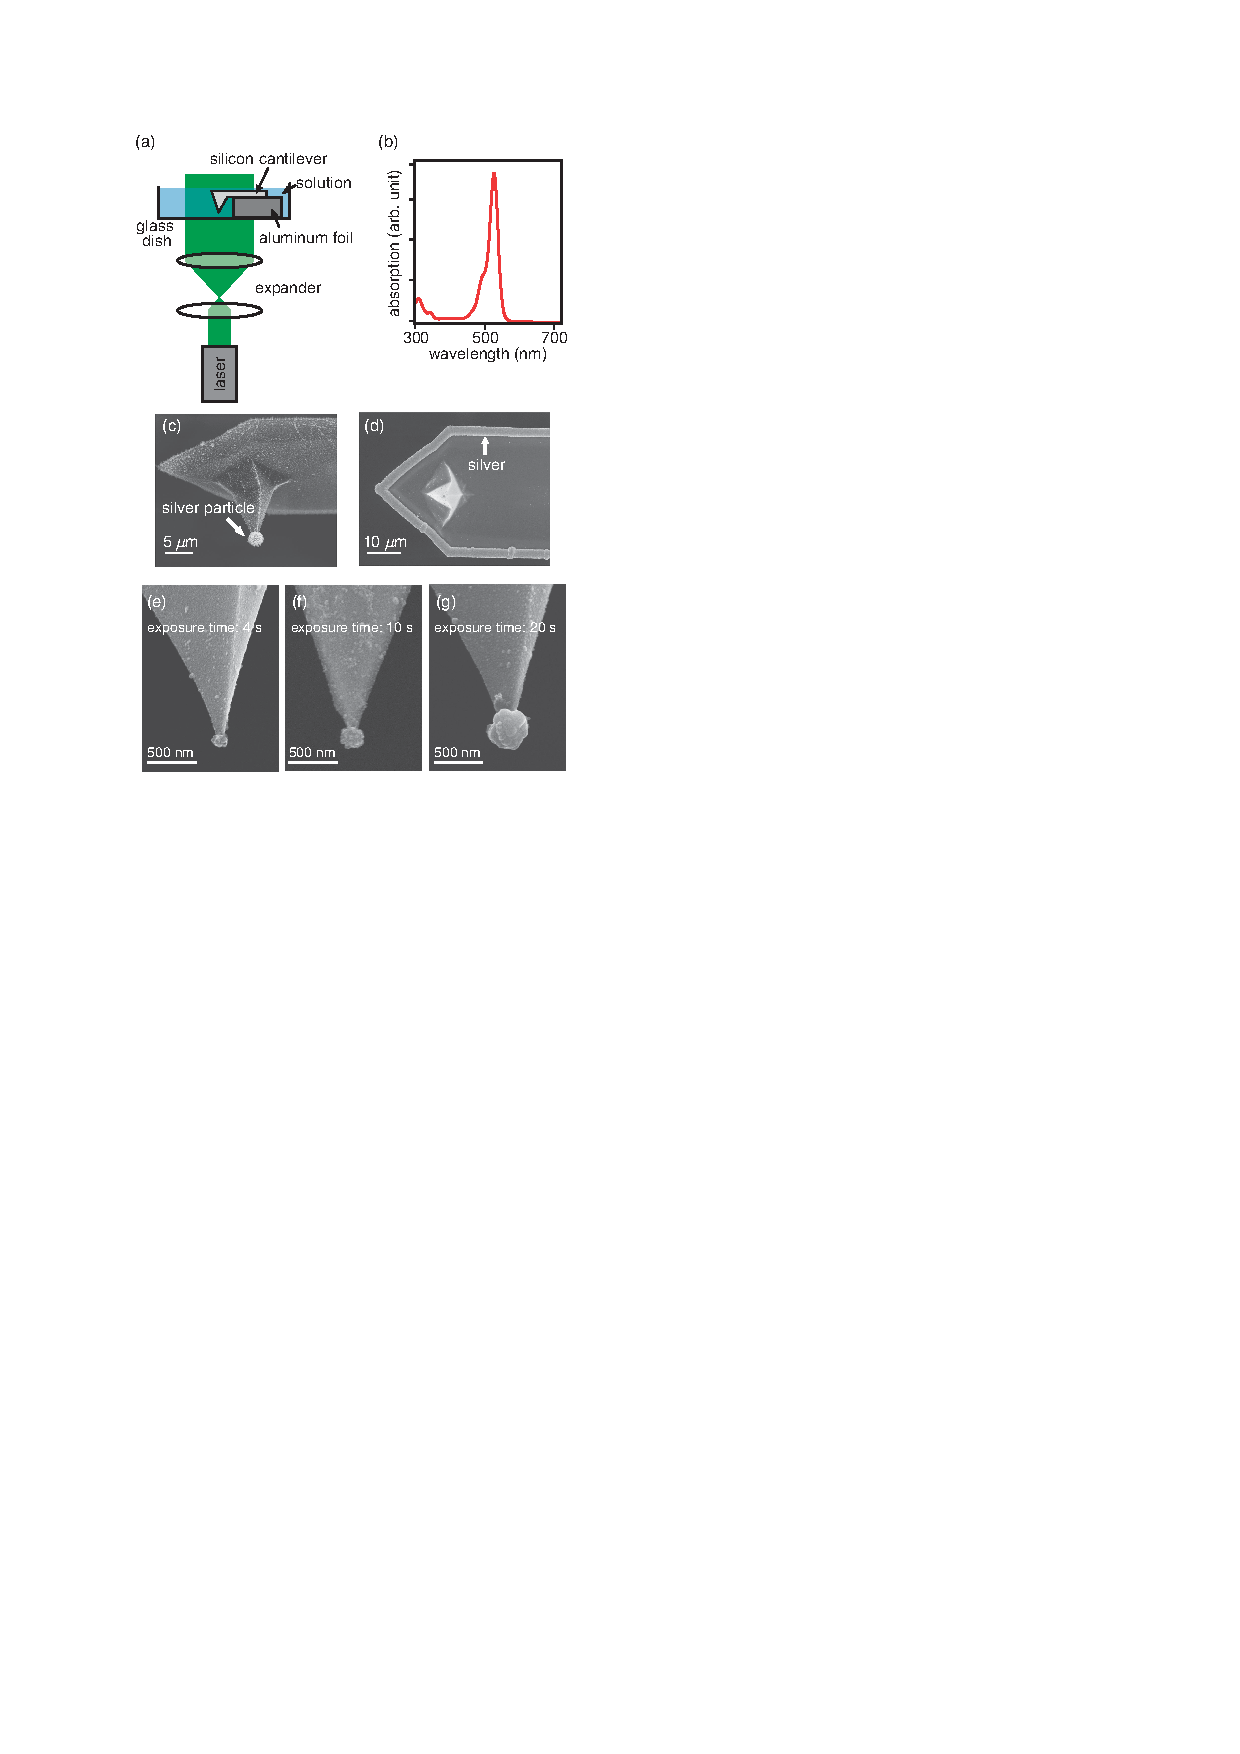
\includegraphics[width=\textwidth, clip=true, trim=0 0 0 130]{figures/literature/umakoshi2012a}
\end{subfigure}
~
\begin{subfigure}[t]{0.6\textwidth}
	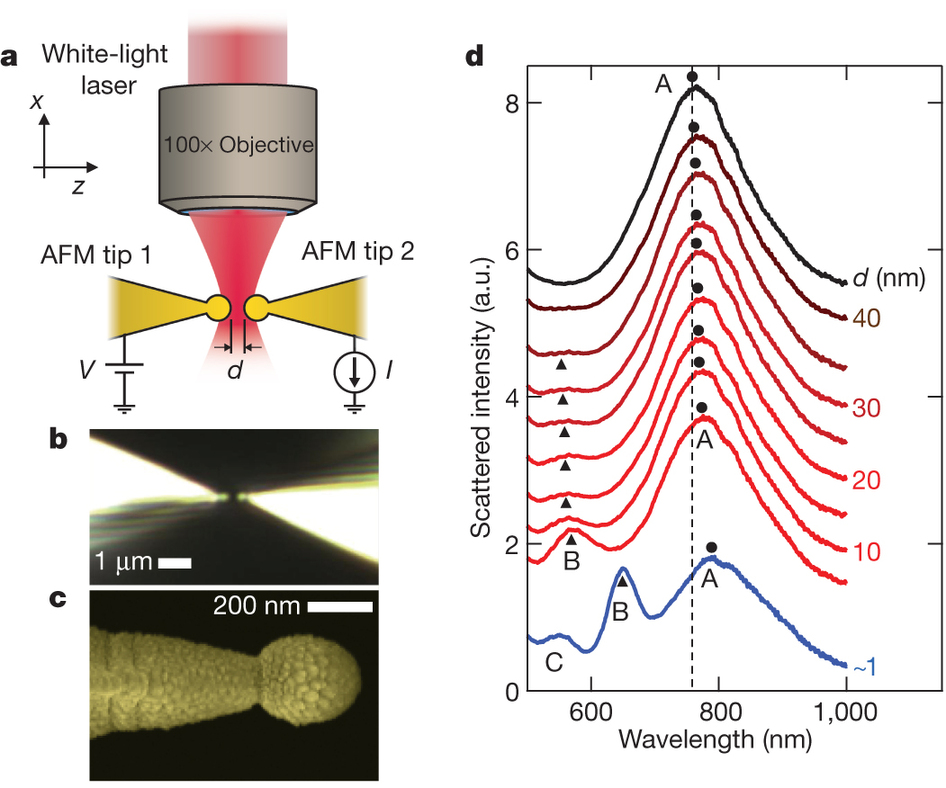
\includegraphics[width=\textwidth, clip=true, trim=0 0 0 40]{figures/literature/nature11653-f1-2}
\end{subfigure}
\caption[Examples of spherical tip fabrication and surface plasmon resonances]{\textbf{Examples of spherical tip fabrication and surface plasmon resonances.} (left) Photochemically fabricated AgNP-on-Si tips for TERS \cite{umakoshi2012}. Field enhancement is increased $\sim$20$\times$ compared with sharp Ag tips when using \SI{488}{nm} illumination with a 1.4\,NA objective in an inverted microscope. (right) Experimental evidence of LSPs in \SI{50}{nm} Au-coated, \SI{150}{nm} radius spherical AFM probes (NanoTools B150) \cite{savage2012}. The large radius minimises sensitivity to axial tip-tip alignment, increases scattered signal levels, and supports higher-order plasmonic cavity modes in the visible spectrum. Resonances are far-field excited using a supercontinuum laser source in a side-illumination configuration. Separation-dependent coupling between two spherical tips confirms plasmonic behaviour.}
\label{fig:savage2012a}
\end{figure}

The simplest geometry to impart onto a tip apex is a sub-wavelength metal sphere. By doing so the tip gains \glspl{lsp} similar to those in an isolated spherical \gls{mnp}. The specific \glspl{spr} depend on the sphere material and geometry along with the attachment method since the base tip structure determines the local adjacent dielectric medium. \Glspl{spr} from spherical Au tips have been previously observed in the far-field \cite{savage2012}, with coupling between plasmons used to confirm plasmonic behaviour, but no characterisation has yet been done. Additionally, a 20$\times$ increase in field enhancement has been measured when using a photochemically-fabricated AgNP-on-Si tip compared with a sharp Ag tip, along with a boost in spatial resolution \cite{umakoshi2012}. These demonstrate that spherical metallic tips have the potential to improve \gls{tenom} if they can be fully understood.

Other than their successful application in \gls{ters} and fundamental plasmonics studies, the origin of \glspl{spr} in spherical tips has not yet been fully investigated. To date there has been very little work done to reliably produce and characterise the optics of spherically nanostructured tips. Furthermore, there is still work needed to similarly measure the optical response of sharp tips, comparing them directly and quantitatively with nanostructured tips. A large part of this project focusses on the development of a simple method for producing plasmonic tips with understood far-field optical responses. The comparison with sharp metallic tips can then be made and plasmonic tips applied in both fundamental studies and near-field enhancement.

\end{document}